\documentclass{article}
\usepackage{graphicx}
\begin{document}
	\section*{Lsg Vorschlag E I Ü011 Maximilian Maag}
	\section*{Aufgabe 11.1}
	\subsection*{a)}
	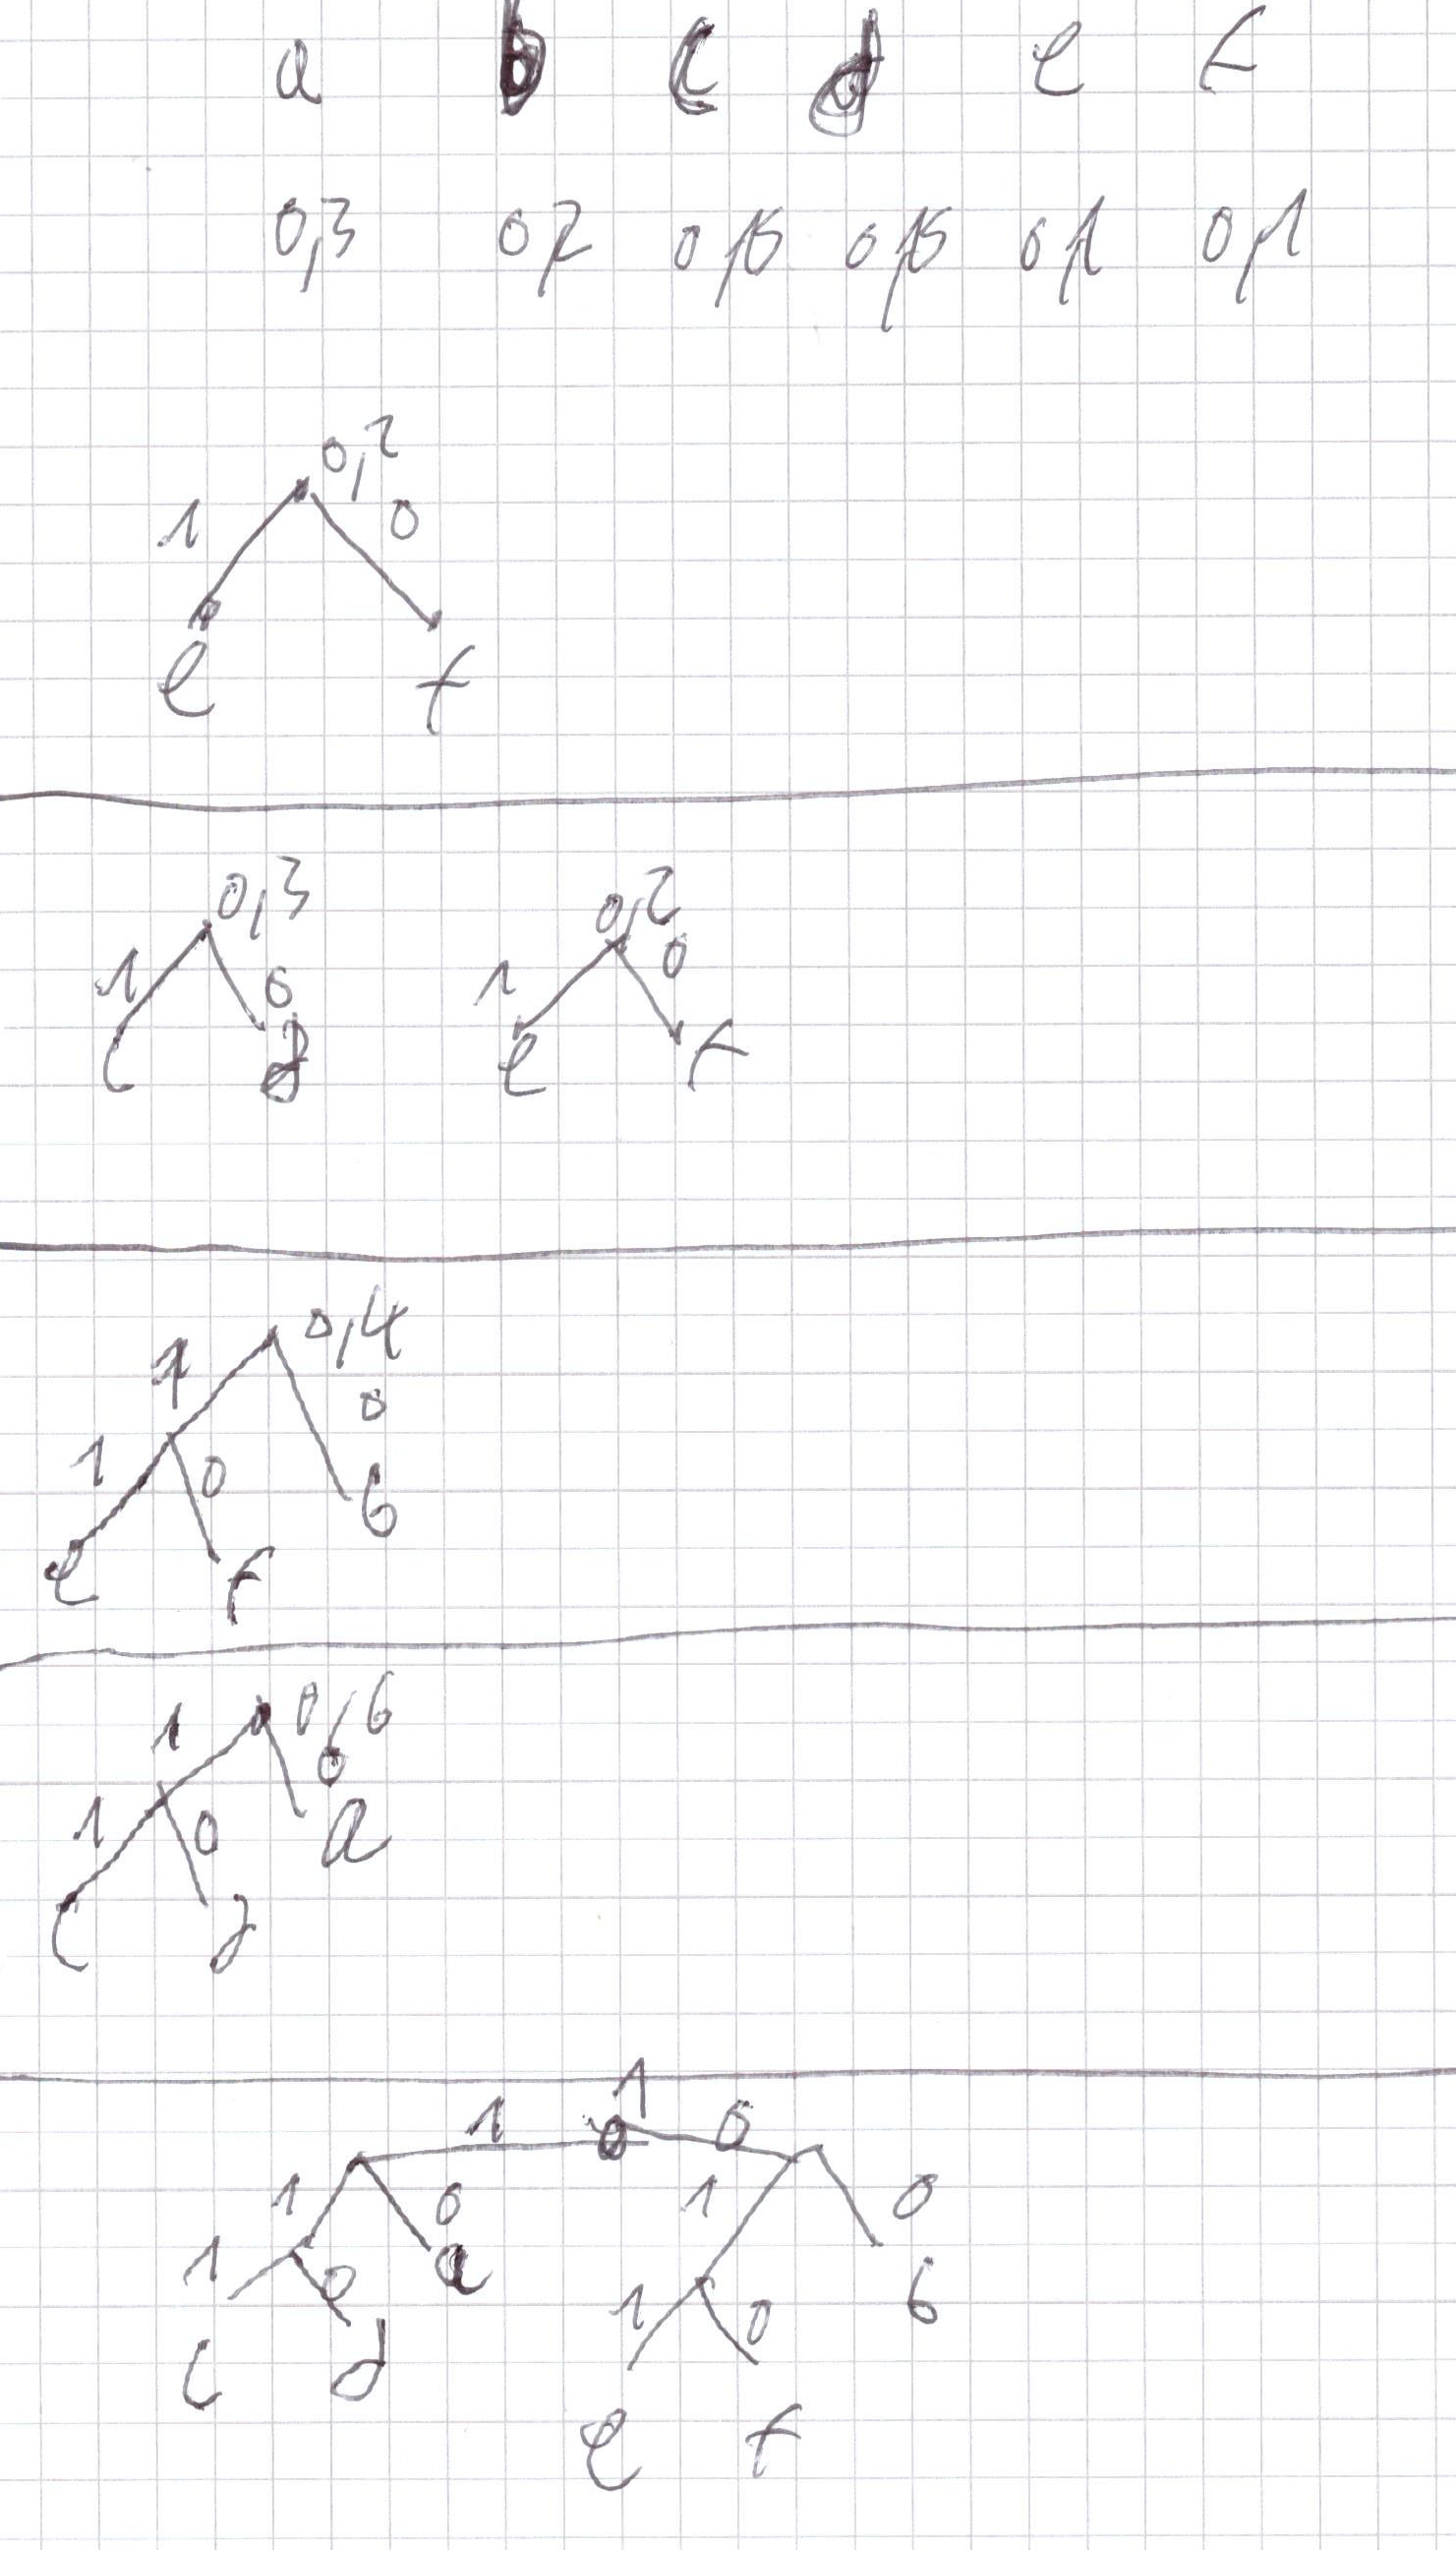
\includegraphics[width=\linewidth, height=\linewidth]{111a}
	\subsection*{b)}
	$L = 2*0,3 + 2*0,3 + 3*0,15 + 3*0,15 + 3*0,1 + 3*0,1$ \\
	$L = 2,7 \approx 3 Byte$
	\subsection*{c)}
	badecfa $\equiv$ 001011001111101010
	\subsection*{d)}
	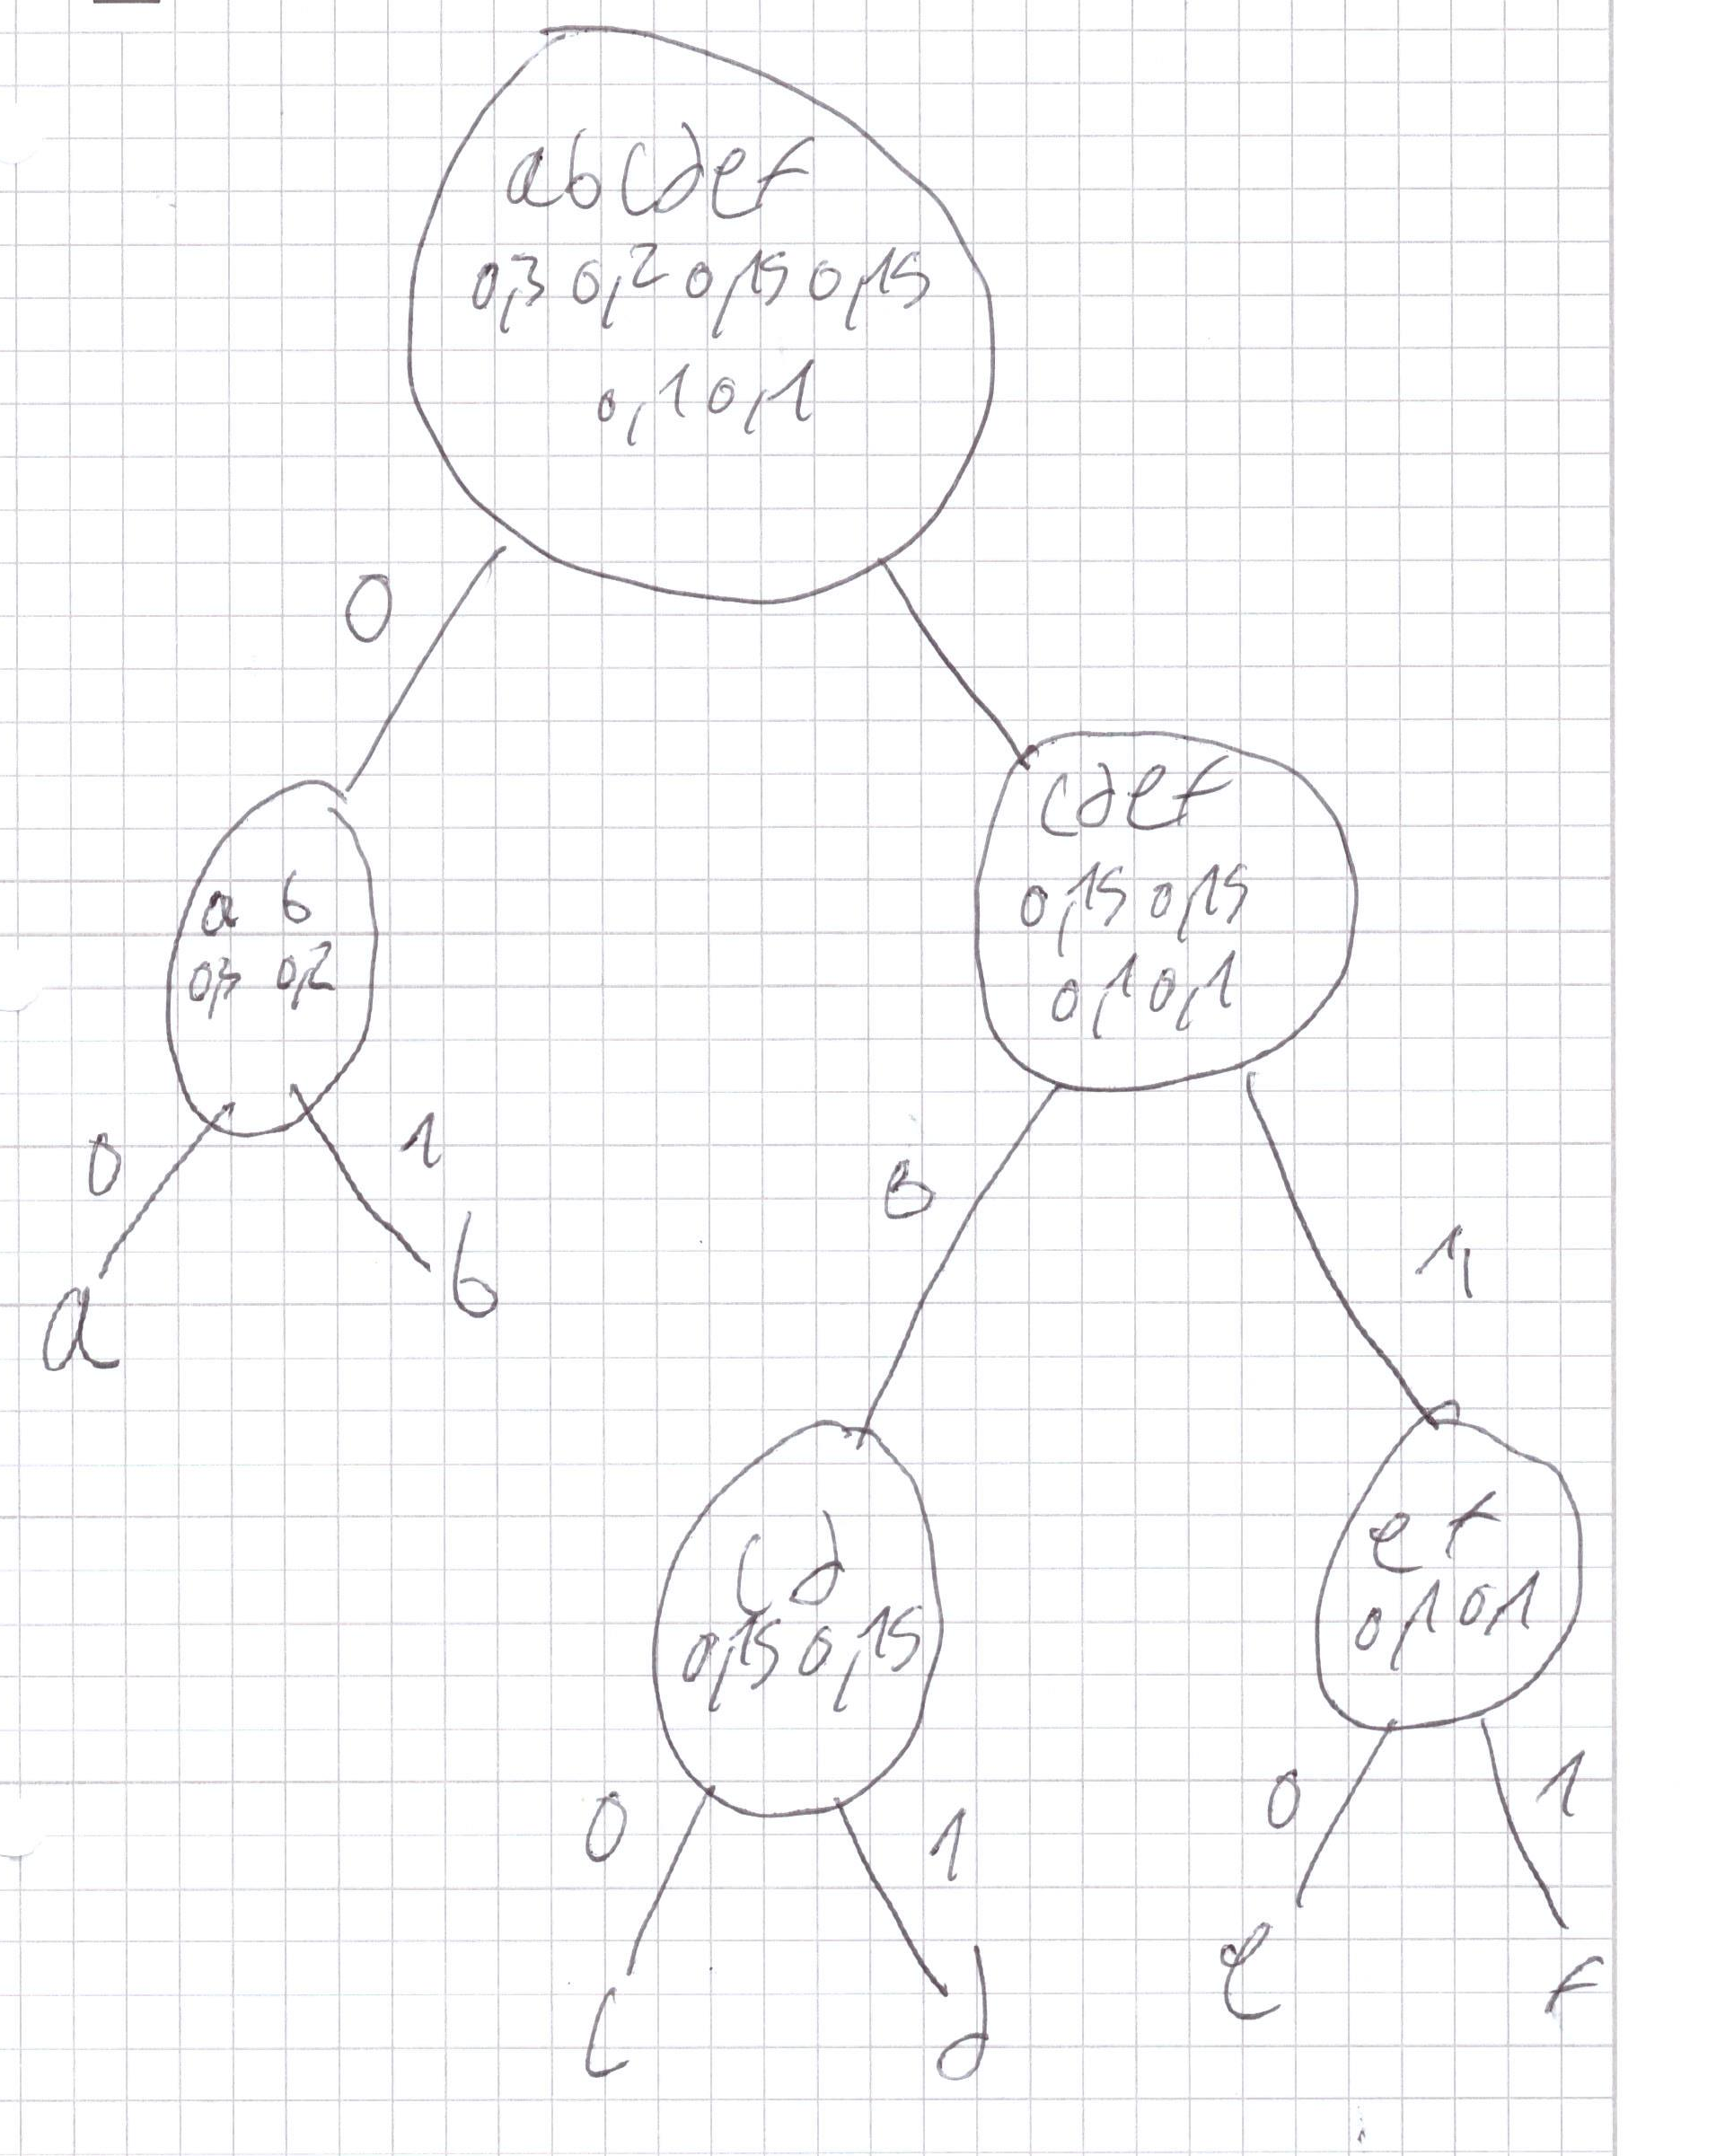
\includegraphics[width=\linewidth]{111d} \\ \\
	badecfa $\equiv$ 010010111010011100 \\
	$L = 2*0,3 + 2*0,2 + 3*0,15 + 3*0,15 + 3*0,1 + 3*0,1$ \\
	$L = 2,5 \approx 3 Byte$
	\section*{Aufgabe 11.2}
	\subsection*{a)}
	Code-Redundanz liegt vor wenn ein Mehraufwand besteht, der über die Darstellung eines Codes hinaus geht. Beispielsweise Pseudotetraden im BCD-Code. \\
	Hamming-Abstand bezeichnet die Anzahl von Stellen an denen sich zwei Codewörter unterscheiden, für einen Code den kleinsten nehmen.
	\subsection*{b)}
	Für die ERKENNUNG von Fehlern muss der Hamming-Abstand um eins Größer sein als die Zahl fehlerhafter Bits. Also für 1-Bitfehler d = 2 und für 3-Bitfehler d = 4.
	\subsection*{c)}
	Bei einem Hamming-Abstand von d = 2k+1 können k-Bitfehler behoben werden. Also für 3-Bitfehler d = 7 und für 1-Bitfehler d = 3.
	
	\section*{Aufgabe 11.3}
	\subsection*{a)}
	Der Hamming-Abstand des Codes erhöht sich auf 2, daher können 1-Bitfehler sicher erkannt werden.
	\subsection*{b)}
	Codewort:Paritätsbit \\
	0010010:0 \\
	1111111:1 \\
	1010101:0 \\
	0001000:1
	\subsection*{c)}
	00100101: Es können nur ungerade Bitfehler erkannt werden. es kann ein 1,3,5 oder 7-Bitfehler sein. \\
	11111111: Damit ein Fehler erkannt wird muss eine gerade Anzahl Bits umklappen. Daraus folgt: 2,4,6 oder 8-Bitfehler.
	\subsection*{d)}
	00100101: gerade Parität ist nicht erfüllt. 1-Bitfehler. \\
	11111111: korrekt übertragen. 
	\section*{Aufgabe 11.4}
	\subsection*{a)}
	3*1+ 5*2+2*3+8*4+0*5+5*6+7*7+8*8+3*9 = 221 \\
	221 mod 11 $\neg$ 6 \\
	3*1+ 5*2+2*3+8*4+0*5+5*6+7*7+3*8+8*9 = 226 \\
	226 mod 11 = 6
	\subsection*{b)}
	2+8*3+1+2*3+3+4*3+5+5*3+4+3*3+2 = 86 \\
	x = 90 - 86 \\
	x = 4 \\
	GTIN: 281234554327
	\section*{Aufgabe 11.5}
	\subsection*{a)}
	Bei der Übertragung ist ein 1-Bitfehler aufgetreten. \\
	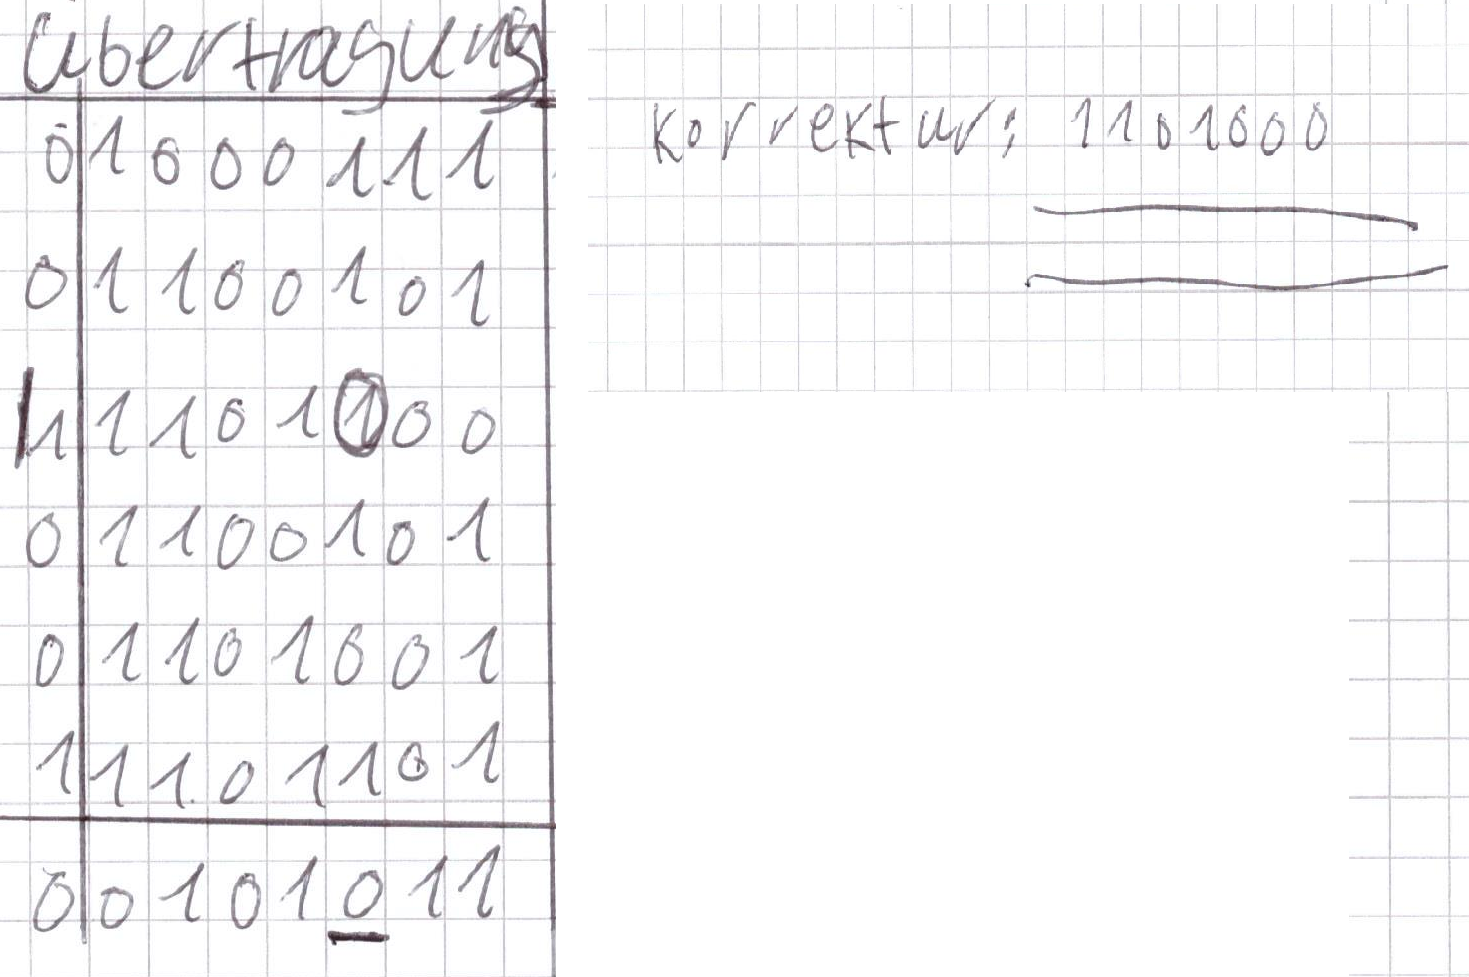
\includegraphics[width=\linewidth]{115a}
	\subsection*{b)}
	\begin{tabular}[h]{c|c}
		binär &  Ascii \\
		\hline
		01000111 & G \\
		01100101 & e\\
		11101100& h \\
		01100101 & e \\
		01101001 & i\\
		11101101 & m
	\end{tabular}
\end{document}